% Options for packages loaded elsewhere
\PassOptionsToPackage{unicode}{hyperref}
\PassOptionsToPackage{hyphens}{url}
\PassOptionsToPackage{dvipsnames,svgnames,x11names}{xcolor}
%
\documentclass[
]{article}
\usepackage{amsmath,amssymb}
\usepackage{lmodern}
\usepackage{iftex}
\ifPDFTeX
  \usepackage[T1]{fontenc}
  \usepackage[utf8]{inputenc}
  \usepackage{textcomp} % provide euro and other symbols
\else % if luatex or xetex
  \usepackage{unicode-math}
  \defaultfontfeatures{Scale=MatchLowercase}
  \defaultfontfeatures[\rmfamily]{Ligatures=TeX,Scale=1}
  \setmainfont[]{fouriernc}
\fi
% Use upquote if available, for straight quotes in verbatim environments
\IfFileExists{upquote.sty}{\usepackage{upquote}}{}
\IfFileExists{microtype.sty}{% use microtype if available
  \usepackage[]{microtype}
  \UseMicrotypeSet[protrusion]{basicmath} % disable protrusion for tt fonts
}{}
\makeatletter
\@ifundefined{KOMAClassName}{% if non-KOMA class
  \IfFileExists{parskip.sty}{%
    \usepackage{parskip}
  }{% else
    \setlength{\parindent}{0pt}
    \setlength{\parskip}{6pt plus 2pt minus 1pt}}
}{% if KOMA class
  \KOMAoptions{parskip=half}}
\makeatother
\usepackage{xcolor}
\usepackage[margin=1in]{geometry}
\usepackage{graphicx}
\makeatletter
\def\maxwidth{\ifdim\Gin@nat@width>\linewidth\linewidth\else\Gin@nat@width\fi}
\def\maxheight{\ifdim\Gin@nat@height>\textheight\textheight\else\Gin@nat@height\fi}
\makeatother
% Scale images if necessary, so that they will not overflow the page
% margins by default, and it is still possible to overwrite the defaults
% using explicit options in \includegraphics[width, height, ...]{}
\setkeys{Gin}{width=\maxwidth,height=\maxheight,keepaspectratio}
% Set default figure placement to htbp
\makeatletter
\def\fps@figure{htbp}
\makeatother
\setlength{\emergencystretch}{3em} % prevent overfull lines
\providecommand{\tightlist}{%
  \setlength{\itemsep}{0pt}\setlength{\parskip}{0pt}}
\setcounter{secnumdepth}{-\maxdimen} % remove section numbering
\newlength{\cslhangindent}
\setlength{\cslhangindent}{1.5em}
\newlength{\csllabelwidth}
\setlength{\csllabelwidth}{3em}
\newlength{\cslentryspacingunit} % times entry-spacing
\setlength{\cslentryspacingunit}{\parskip}
\newenvironment{CSLReferences}[2] % #1 hanging-ident, #2 entry spacing
 {% don't indent paragraphs
  \setlength{\parindent}{0pt}
  % turn on hanging indent if param 1 is 1
  \ifodd #1
  \let\oldpar\par
  \def\par{\hangindent=\cslhangindent\oldpar}
  \fi
  % set entry spacing
  \setlength{\parskip}{#2\cslentryspacingunit}
 }%
 {}
\usepackage{calc}
\newcommand{\CSLBlock}[1]{#1\hfill\break}
\newcommand{\CSLLeftMargin}[1]{\parbox[t]{\csllabelwidth}{#1}}
\newcommand{\CSLRightInline}[1]{\parbox[t]{\linewidth - \csllabelwidth}{#1}\break}
\newcommand{\CSLIndent}[1]{\hspace{\cslhangindent}#1}
\newcommand{\indep}{\perp \!\!\! \perp}
\usepackage[T1]{fontenc}
\usepackage{fouriernc}
\usepackage{setspace}\onehalfspacing
\usepackage{amsfonts}
\usepackage{dcolumn}
\usepackage{pifont}
\usepackage{booktabs}
\usepackage{placeins}
\usepackage{caption}
\usepackage{fancyhdr}
\pagestyle{fancy}
\fancyhf{}
\rhead{Final AVCD assignment}
\lhead{1050713}
\renewcommand{\headrulewidth}{0pt}
\cfoot{\thepage}
\usepackage{booktabs}
\usepackage{longtable}
\usepackage{array}
\usepackage{multirow}
\usepackage{wrapfig}
\usepackage{float}
\usepackage{colortbl}
\usepackage{pdflscape}
\usepackage{tabu}
\usepackage{threeparttable}
\usepackage{threeparttablex}
\usepackage[normalem]{ulem}
\usepackage{makecell}
\usepackage{xcolor}
\usepackage{siunitx}

  \newcolumntype{d}{S[
    input-open-uncertainty=,
    input-close-uncertainty=,
    parse-numbers = false,
    table-align-text-pre=false,
    table-align-text-post=false
  ]}
  
\ifLuaTeX
  \usepackage{selnolig}  % disable illegal ligatures
\fi
\IfFileExists{bookmark.sty}{\usepackage{bookmark}}{\usepackage{hyperref}}
\IfFileExists{xurl.sty}{\usepackage{xurl}}{} % add URL line breaks if available
\urlstyle{same} % disable monospaced font for URLs
\hypersetup{
  pdftitle={Economic insecurity, lack of representation and radical-right voting in the context of the 2021 German federal election},
  pdfauthor={Candidate number: 1050713},
  colorlinks=true,
  linkcolor={gray},
  filecolor={Maroon},
  citecolor={Blue},
  urlcolor={magenta},
  pdfcreator={LaTeX via pandoc}}

\title{Economic insecurity, lack of representation and radical-right
voting in the context of the 2021 German federal election}
\author{Candidate number: 1050713}
\date{26 May 2023}

\begin{document}
\maketitle

\hypertarget{introduction}{%
\section{Introduction}\label{introduction}}

This essay examines whether, as some argue, the association between
economic insecurity and radical-right support is moderated by voters'
sense that the political system is incapable of addressing their
economic grievances. To that end, I will, first, contextualise this
research question in relation to the relevant literature, and, secondly,
discuss the operationalisation of my dependent and independent
variables. Thirdly, I will present my methodology and results, which do
\emph{not} support the argument that the political system's perceived
lack of responsiveness moderates the relationship between economic
insecurity and radical-right voting in the context of the 2021 German
federal election.

\hypertarget{motivation}{%
\section{Motivation and relation to literature}\label{motivation}}

2023 marks the tenth year of the \emph{Alternative für Deutschland}'s
(AfD) existence. Originally founded by a coterie of eurosceptic
professors, the AfD had, by late 2015, morphed into a classic
radical-right party, when it started to adopt a strongly nativist,
anti-immigrant platform
(\protect\hyperlink{ref-arzheimer_how_2019}{Arzheimer and Berning 2019};
\protect\hyperlink{ref-cantoni_persistence_2020}{Cantoni, Hagemeister,
and Westcott 2020}). The AfD's entry into the \emph{Bundestag} in 2017
was part of the wave of populist success that many (Western) European
countries witnessed during the mid-2010s. This wave led to the debate
about the determinants of radical-right support -- which had been
ongoing among political scientists at least since the late 1990s (e.g.
\protect\hyperlink{ref-kitschelt_radical_1995}{Kitschelt and McGann
1995}) -- gaining greater attention in both other disciplines
(\protect\hyperlink{ref-guriev_political_2022}{Guriev and Papaioannou
2022}) and public discourse.

While much of the debate on the demand-side of radical-right voting has
focused on the relative importance of economic and cultural factors
respectively (\protect\hyperlink{ref-colantone_surge_2019}{Colantone and
Stanig 2019}; \protect\hyperlink{ref-margalit_economic_2019}{Margalit
2019}; \protect\hyperlink{ref-art_myth_2022}{Art 2022};
\protect\hyperlink{ref-margalit_cultural_2022}{Margalit, Raviv, and
Solodoch 2022}), the theoretical framework I test below belongs to
another, somewhat more nascent strand of the literature. This strand
argues, inter alia, that the effect of economic grievances is moderated
by (i) voters' trust in political institutions, notably parties and
parliaments, and (ii) the degree to which they feel their preferences
are represented in the party system (e.g.
\protect\hyperlink{ref-dustmann_europes_2017}{Dustmann et al. 2017};
\protect\hyperlink{ref-eichengreen_populist_2018}{Eichengreen 2018};
\protect\hyperlink{ref-ivanov_economic_2023}{Ivanov 2023}).

Though often not explicitly acknowledged by non-political-scientists,
this set of theoretical hypotheses echoes not only the work by Katz and
Mair (\protect\hyperlink{ref-katz_cartel_2009}{2009}) on the
cartelisation of Western European party systems, but also more recent
work stressing the importance of representational deficits in driving
populist support (e.g.
\protect\hyperlink{ref-manow_ent-demokratisierung_2020}{Manow 2020};
\protect\hyperlink{ref-schafer_demokratische_2021}{Schäfer and Zürn
2021}; \protect\hyperlink{ref-silva_parties_2023}{Silva and Wratil
2023}). More importantly, these hypotheses have been subjected to
relatively little empirical testing, as Sonin
(\protect\hyperlink{ref-sonin_historical_2022}{2022}) notes in his
review of the work by Eichengreen
(\protect\hyperlink{ref-eichengreen_populist_2018}{2018}). This essay is
intended as a small step towards filling this gap in the literature.

\hypertarget{theory}{%
\section{Theory and case selection}\label{theory}}

Like many economic-insecurity-centred accounts of radical-right support,
the theoretical argument starts from the observation that economic
shocks - such as automation
(\protect\hyperlink{ref-boix_democratic_2019}{Boix 2019}) and trade
liberalisation (\protect\hyperlink{ref-autor_china_2013}{Autor, Dorn,
and Hanson 2013}) - create winners and losers. This assumption holds
true not only for most Western European countries
(\protect\hyperlink{ref-colantone_trade_2018}{Colantone and Stanig
2018a}; \protect\hyperlink{ref-milner_voting_2021}{Milner 2021}), in
general, but also for Germany, in particular
(\protect\hyperlink{ref-dauth_rise_2014}{Dauth, Findeisen, and Südekum
2014}; \protect\hyperlink{ref-dauth_adjustment_2021}{Dauth et al.
2021}). Those losers, the argument goes on, who do not believe the
current political system can address their grievances will then turn to
populist radical-right parties.

By way of unpacking this argument, note, first, that losers may believe
the political system to be incapable of redressing their economic
grievances for two distinct reasons. First, they might deem all
mainstream parties to be much of a muchness, meaning none of the
supposedly different parties is seen by losers as representing their
preferences. In that instance, losers are likely to think that it does
not matter which mainstream party they vote for, or which of those
parties governs. Second, even if voters believe at least one mainstream
party to endorse policies conducive to redressing their economic
grievances, they might not trust any mainstream politician to follow
through on these promises.\footnote{This `trust' channel is distinct
  from a `valence' channel, where voters fundamentally trust
  politicians, but judge their levels of competence to differ
  (\protect\hyperlink{ref-green_politics_2017}{Green and Jennings
  2017}).}

These two reasons also show why the theory predicts economic losers, as
a result of their grievances, to turn to radical-right parties, rather
than left-wing parties. Many other economic-insecurity-type arguments
are unable to resolve this puzzle, which arises because the latter's
platforms tend to be significantly more pro-redistributive than the
former's platforms. Using the terminology introduced by Linz
(\protect\hyperlink{ref-linz_breakdown_1978}{1978}), the reason is that
losers regard left-wing parties as loyal to the political system and in
cahoots with the other mainstream actors. Their redistributive promises
therefore lack credibility. By contrast, radical-right parties'
semi-loyalty or outright disloyalty to the system means that voting for
them increases the likelihood that the political system, characterised
by the mainstream cartel (\protect\hyperlink{ref-katz_cartel_2009}{Katz
and Mair 2009}), will be disrupted.

In sum, this theoretical argument implies (at least)\footnote{The
  argument could also be taken to imply that (i) a perceived lack of
  representation and (ii) low trust increase the probability of voting
  for the radical right. Given the space constraints, I prescind from
  testing these two hypotheses.} four testable hypotheses.

\begin{itemize}
\tightlist
\item
  H1: Economic insecurity, \emph{ceteris paribus}, increases the
  probability of voting for the radical right.
\item
  H2: The effect of economic insecurity on the probability of voting for
  the radical right is, \emph{ceteris paribus}, stronger for those who
  believe their preferences not be represented in the current party
  system.
\item
  H3: The effect of economic insecurity is, \emph{ceteris paribus},
  stronger for those who are more distrustful of parties and/or
  parliament.
\item
  H4: Economic insecurity, \emph{ceteris paribus}, increases the
  probability of voting for the radical right, relative to
  pro-redistributive left-wing parties, notably the SPD and LINKE.
\end{itemize}

Before setting out my empirical strategy, let me briefly discuss my two
reasons for choosing the case of the 2021 German federal election.
First, the 2021 election occurred in the wake of the third wave of the
Covid-19 pandemic, which caused widespread financial insecurity among
German households
(\protect\hyperlink{ref-cziriak_publication_nodate}{Cziriak 2022}).
Secondly, the pandemic was a politically contentious period, causing
deep divides over the desirability and efficacy of both
non-pharmaceutical interventions, such as mask mandates, and
vaccination. The \emph{Querdenker} movement, in particular, used their
protests to stress that their interests were not represented by any
mainstream party (e.g.
\protect\hyperlink{ref-plumper_strategy_2021}{Plümper, Neumayer, and
Pfaff 2021}). Both factors mean that economic insecurity and
subjectively perceived representational deficits were likely salient in
the minds of some voters, making this election a suitable case for
testing the above hypotheses.

\hypertarget{data-variables-and-operationalisation}{%
\section{Data, variables and
operationalisation}\label{data-variables-and-operationalisation}}

To test the above hypotheses, I use the \emph{German Longitudinal
Election Study's} (GLES)
\href{https://search.gesis.org/research_data/ZA7701}{2021 post-election
survey} - a high-quality survey of a cross-section of 3424
(quasi-)randomly selected individuals, containing a rich set of
questions about respondents' social and political attitudes as well as
their socio-demographic characteristics. The survey was conducted
shortly after the federal election.\footnote{The federal election was
  held on 26 September 2021, while the survey was conducted between 27
  September 2021 and 21 November 2021.} We therefore get to observe
respondents' (self-reported) voting behaviour, rather than merely their
voting intention, while reducing the risk of recall problems biasing our
results. That said, this survey, like most others, faces the limitation
that we cannot rule out that respondents' actual voting behaviour
diverges from their self-reported one.

\begin{table}[!h]

\caption{\label{tab:data-summary-table}Summary of variables and their operationalisation}
\centering
\resizebox{\linewidth}{!}{
\fontsize{11}{13}\selectfont
\begin{tabular}[t]{lll}
\toprule
Variable & Operationalisation & Survey item(s)\\
\midrule
\addlinespace[0.3em]
\multicolumn{3}{l}{\textbf{dependent variable}}\\
\hspace{1em}Radical-right voting & factor indicating party vote choice & q114ba\\
\hspace{1em} & dummy for AfD Zweitstimme & q114ba = 322\\
\addlinespace[0.3em]
\multicolumn{3}{l}{\textbf{independent variables}}\\
\hspace{1em}Economic insecurity & dummy for unemployment in past ten years & d17a-c\\
\hspace{1em} & fear of job loss & d18\\
\hspace{1em} & fear of losing or having to change profession & d19\\
\hspace{1em} & personal economic situation currently & q13\\
\hspace{1em}Political system not responsive & no difference which party governs & q117\\
\hspace{1em} & no difference which party one votes for & q118\\
\hspace{1em}Trust in political system & trust in parliament & q79b\\
\hspace{1em} & trust in parties & q79c\\
\bottomrule
\multicolumn{3}{l}{\textsuperscript{*} Unemployment experience is, following Dauth et al (2021), defined as an individual having}\\
\multicolumn{3}{l}{been unemployed for at least one year.}\\
\multicolumn{3}{l}{\textsuperscript{*} Source: Codebook for GLES Cross-Section 2021, Post-Election, ZA7701, Dataset Version v1.0.0.}\\
\end{tabular}}
\end{table}

My dependent variable is radical-right voting, which, in the German
context, means casting one's party vote (\emph{Zweitstimme}) for the
AfD. As indicated in table 1, I operationalise the dependent variable in
two ways. I use a dummy variable to test hypotheses H1 to H3, while I
rely on the full factor variable to test H4. This is because the first
three hypotheses concern the probability of voting for the radical
right, relative to all other parties, whereas the fourth hypothesis
concerns the probability of voting for the AfD, relative to the
pro-redistributive, left-wing parties, the SPD and LINKE.

My independent variables of interest are economic insecurity,
respondents' perception of the political system's responsiveness, and
their trust in the system. To operationalise economic insecurity, I use
a dummy for actual unemployment experience in the past ten years. Given
that the labour market literature shows past unemployment to be strongly
predictive of present unemployment risk (e.g.
\protect\hyperlink{ref-autor_unexpected_2023}{Autor, Dube, and McGrew
2023}), this dummy can be interpreted as an objective measure of
economic insecurity. To capture subjectively perceived insecurity, I
rely on respondents' fear of losing their jobs in the next two years.
The other two economic insecurity variables (see table 1) are merely
used to probe the robustness of my findings (see
\protect\hyperlink{appendix}{appendix}). Finally, following
(\protect\hyperlink{ref-colantone_global_2018}{Colantone and Stanig
2018b}), I use respondents' answers to the questions `Does it make a
difference who is governing/who one votes for?' and `How much do you
trust parliament/political parties?' as measures for the perceived
responsiveness of Germany's political system and voters' trust in the
latter respectively.

\hypertarget{methodology-and-results}{%
\section[Methodology and results]{\texorpdfstring{Methodology\footnote{The
  replication code can be found
  \href{https://github.com/jacob-edenhofer/Analysing_Vote_Choice_Data_TT2023}{here}.}
and results}{Methodology and results}}\label{methodology-and-results}}

I estimate logistic regressions to test the first three hypotheses since
my dependent variable is a dummy for AfD party vote. I regress the
latter on my two measures for economic insecurity as well as the
measures for representation and trust, and the interactions between them
and economic insecurity. In addition, I include a vector of covariates
to control for potential observable confounders. The vector includes
respondents' household income, their age, education, the rurality of
their place of residence and a dummy indicating whether they currently
live in East or West German states.

Save for the East-West dummy and, possibly, the rurality variable, these
are standard covariates in the literature, with, for instance, Colantone
and Stanig (\protect\hyperlink{ref-colantone_surge_2019}{2019})
explaining why these might confound the relationship between economic
insecurity and radical-right voting. The inclusion of the rurality
variable is motivated by the work of Haffert
(\protect\hyperlink{ref-haffert_stadt_2022}{2022}), who shows that
geographic location has become an important determinant of voting
behaviour in Germany in recent years. The East-West dummy accounts for
the economic, cultural, and political differences between these two
parts of Germany (e.g.
\protect\hyperlink{ref-becker_2020_separation}{Becker, Mergele, and
Wößmann 2020}). Letting \(\textbf{X}\) denote the vector of covariates
and \(\epsilon\) the error term, we can write the estimating
equation\footnote{The specification for trust is entirely analogous.}
for the logistic regression with the political system's responsiveness
as the moderating variable as follows:

\[
log(\frac{AfD_{i}}{1-AfD_{i}}) = \alpha + \beta_{1}Insecurity_{i} +  \beta_{2}Representation_{i} + \beta_{3}Insecurity_{i}*Representation_{i} + \beta_{4}\textbf{X}_{i} + \epsilon_{i}
\]

Figure 1 visualises\footnote{See tables 2 and 3 in the
  \protect\hyperlink{appendix}{appendix} for the full regression tables,
  including coefficient estimates for the covariates.} the results from
estimating these specifications. H1, H2 and H3 imply that
\(\beta_{1}>0\) and \(\beta_{3}>0\). Using the unemployment experience
and fear of job loss variables as proxies for economic insecurity,
figure 1 shows that, contrary to expectations, economic insecurity does
\emph{not} significantly increase the probability of voting for the AfD.
The coefficient estimates on the interaction terms are, except for one,
statistically insignificant, suggesting it is \emph{not} the case that
the marginal effect of insecurity varies by the political system's
responsiveness or respondents' trust in parliament. This conclusion is
reinforced by figures 2 and 3 in the
\protect\hyperlink{appendix}{appendix}. Finally, this null finding is
largely,\footnote{Two of the interaction terms in table 7 are
  statistically significant.} as tables 5 and 6 in the
\protect\hyperlink{appendix}{appendix} bear out, robust to relying on
the two other proxies for economic insecurity mentioned in table 1.

\begin{figure}
\centering
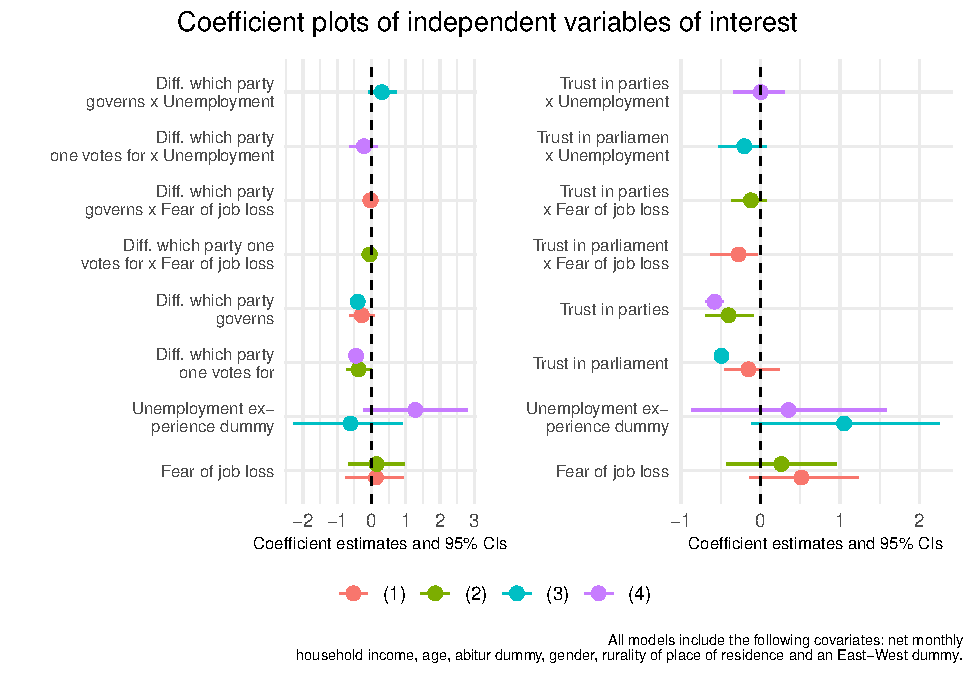
\includegraphics{AVCD_Final-Assignment-1050713_files/figure-latex/regression-results1-plot-1.pdf}
\caption{Summary of tests for H1 - H3}
\end{figure}

Testing H4 requires us to modify our estimation technique to account for
the dependent variable being a multi-category factor, rather than a
dichotomous variable. To that end, I estimate a multinomial model, using
the same vector of covariates as above. Respondents' fear of losing
their jobs serves as my proxy for economic insecurity and their answers
to the question `Does it make a difference who is governing?' as my
measure for the political system's responsiveness. I also drop the
interaction term since H4 is \emph{not} about differences in marginal
effects, i.e.:

\[
RelativeProbability_{ij} = \alpha + \beta_{1}Insecurity_{i} +  \beta_{2}Representation_{i} + \beta_{3}\textbf{X}_{i} + \epsilon_{i}
\]

The dependent variable indicates the probability that respondent \(i\)
votes for party \(j\), rather than voting for the AfD. As explained
above, H4 implies that \(\beta_{1}\) should be negative for the SPD and
LINKE.

\begin{figure}
\centering
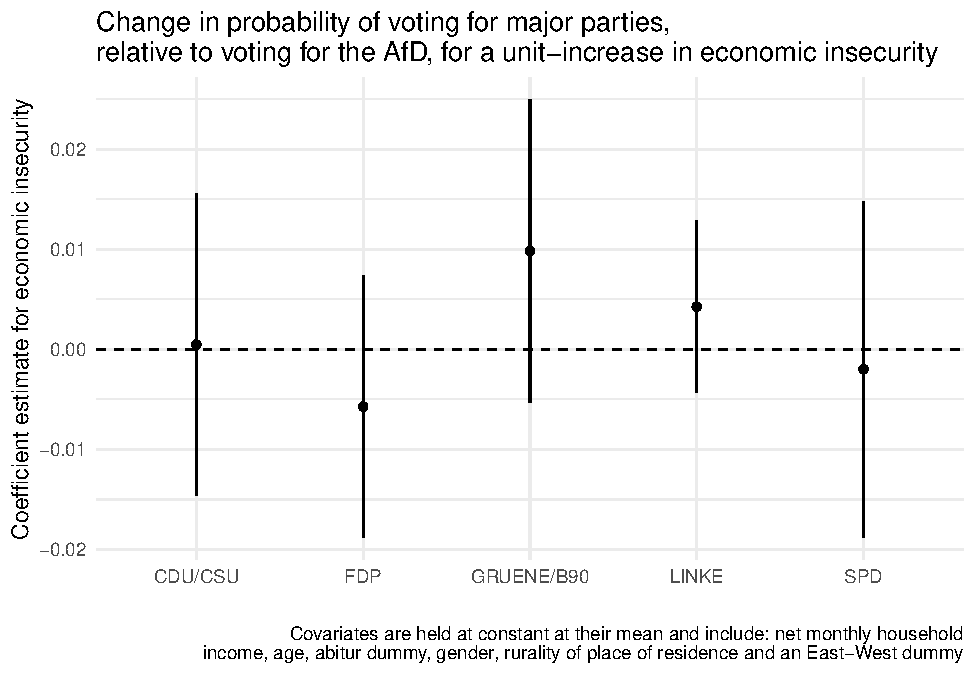
\includegraphics{AVCD_Final-Assignment-1050713_files/figure-latex/multinomial-model-plot-1.pdf}
\caption{Coefficient estimate of economic insecurity from multinomial
model}
\end{figure}

Figure 2 shows the coefficient estimates\footnote{See table 4 in
  \protect\hyperlink{appendix}{appendix} for the full regression table.}
for \(\beta_{1}\) - none of which are statistically significant at
conventional levels.\footnote{Conventional levels being the 1\%, 5\% and
  10\% levels.} This entails that a unit-increase in economic insecurity
does not significantly reduce the relative probability of voting for
pro-redistributive, left-wing parties, here the SPD and Linke. Hence, we
find no support for H4.

Before concluding, it is worth dwelling on two limitations of the above
analysis. First, the regression results should not be interpreted
causally. While I control for a set of observable confounders, I cannot
rule out that other variables, particularly unobservable ones, confound
the relationship between economic insecurity and radical-right voting.
Second, my measures for the key independent variables (see table 1),
particularly economic insecurity, are noisy, which can complicate
statistical inference by inflating standard errors and, thus, increasing
the risk of type II errors or null results.

\hypertarget{conclusion}{%
\section{Conclusion}\label{conclusion}}

In summary, I examined whether the German political system's perceived
responsiveness and voter's trust in the latter moderate the relationship
between economic insecurity and AfD support. By estimating a series of
logistic and multinomial regressions models, I found this \emph{not} to
be the case in the 2021 German federal election. While this null finding
is robust to different operationalisations of the key independent
variables, the analysis is subject to considerable limitations, implying
that the results should be interpreted as tentative, rather than
definitive, evidence against the hypotheses tested here.

\emph{Word count: 2098}

\hypertarget{appendix}{%
\section{Appendix}\label{appendix}}

\hypertarget{marginal-effect-plots-and-regression-tables}{%
\subsection{Marginal effect plots and regression
tables}\label{marginal-effect-plots-and-regression-tables}}

\begin{table}[!h]

\caption{\label{tab:regression-results-1-table1}Association between the probability of voting for the AfD and economic insecurity}
\centering
\begin{tabular}[t]{lcccc}
\toprule
  & (1) & (2) & (3) & (4)\\
\midrule
Fear of job loss & \num{0.130} & \num{0.147} &  & \\
 & (\num{0.425}) & (\num{0.407}) &  & \\
Unemployment experience dummy &  &  & \num{-0.613} & \num{1.277}+\\
 &  &  & (\num{0.801}) & (\num{0.767})\\
Difference which party one votes for &  & \num{-0.375}* &  & \num{-0.451}***\\
 &  & (\num{0.187}) &  & (\num{0.077})\\
Difference which party governs & \num{-0.281} &  & \num{-0.402}*** & \\
 & (\num{0.186}) &  & (\num{0.077}) & \\
Difference which party one votes for
x Fear of job loss &  & \num{-0.050} &  & \\
 &  & (\num{0.121}) &  & \\
Difference which party governs
x Fear of job loss & \num{-0.028} &  &  & \\
 & (\num{0.118}) &  &  & \\
Difference which party one votes for
x Unemployment &  &  &  & \num{-0.219}\\
 &  &  &  & (\num{0.211})\\
Difference which party governs
x Unemployment &  &  & \num{0.304} & \\
 &  &  & (\num{0.207}) & \\
Age & \num{-0.009} & \num{-0.010} & \num{-0.008} & \num{-0.009}\\
 & (\num{0.010}) & (\num{0.010}) & (\num{0.005}) & (\num{0.006})\\
Female dummy & \num{-0.778}** & \num{-0.781}** & \num{-0.676}*** & \num{-0.708}***\\
 & (\num{0.252}) & (\num{0.255}) & (\num{0.183}) & (\num{0.187})\\
Household income & \num{-0.123}* & \num{-0.106}+ & \num{-0.097}* & \num{-0.081}*\\
 & (\num{0.060}) & (\num{0.061}) & (\num{0.039}) & (\num{0.040})\\
Rurality of place
of residence & \num{0.241}* & \num{0.243}* & \num{0.092} & \num{0.109}\\
 & (\num{0.117}) & (\num{0.118}) & (\num{0.082}) & (\num{0.084})\\
No Abitur dummy & \num{1.013}*** & \num{0.982}** & \num{0.818}*** & \num{0.773}***\\
 & (\num{0.299}) & (\num{0.303}) & (\num{0.221}) & (\num{0.223})\\
West Germany dummy & \num{-1.385}*** & \num{-1.336}*** & \num{-1.047}*** & \num{-1.017}***\\
 & (\num{0.245}) & (\num{0.248}) & (\num{0.178}) & (\num{0.182})\\
\midrule
Num.Obs. & \num{1276} & \num{1265} & \num{2324} & \num{2296}\\
AIC & \num{548.7} & \num{537.0} & \num{1013.5} & \num{984.9}\\
BIC & \num{600.2} & \num{588.4} & \num{1071.1} & \num{1042.3}\\
Log.Lik. & \num{-264.344} & \num{-258.483} & \num{-496.774} & \num{-482.439}\\
RMSE & \num{0.24} & \num{0.24} & \num{0.24} & \num{0.24}\\
\bottomrule
\end{tabular}
\end{table}

\begin{figure}
\centering
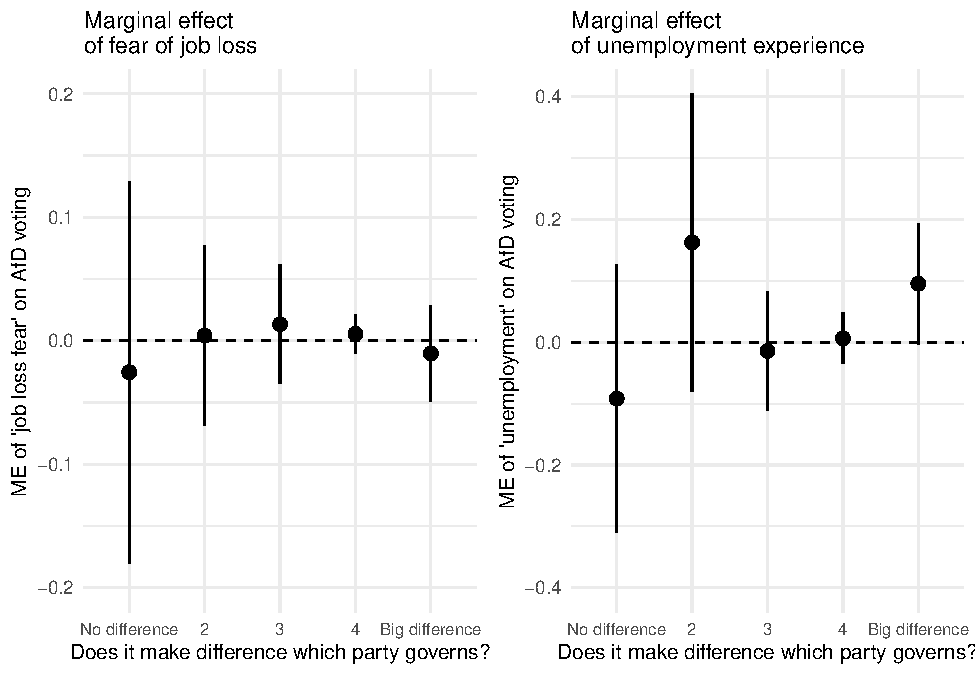
\includegraphics{AVCD_Final-Assignment-1050713_files/figure-latex/regression-results-1-plot1-1.pdf}
\caption{Marginal effects of economic insecurity by perceived
responsiveness}
\end{figure}

\begin{table}[!h]

\caption{\label{tab:regression-results-1-table2}Association between the probability of voting for the AfD and economic insecurity}
\centering
\begin{tabular}[t]{lcccc}
\toprule
  & (1) & (2) & (3) & (4)\\
\midrule
Fear of job loss & \num{0.515} & \num{0.261} &  & \\
 & (\num{0.347}) & (\num{0.348}) &  & \\
Unemployment experience dummy &  &  & \num{1.051}+ & \num{0.352}\\
 &  &  & (\num{0.599}) & (\num{0.621})\\
Trust in parliament & \num{-0.151} &  & \num{-0.491}*** & \\
 & (\num{0.170}) &  & (\num{0.045}) & \\
Trust in parties &  & \num{-0.401}** &  & \num{-0.578}***\\
 &  & (\num{0.155}) &  & (\num{0.059})\\
Trust in parliament
x Fear of job loss & \num{-0.276}+ &  &  & \\
 & (\num{0.150}) &  &  & \\
Trust in parties
x Fear of job loss &  & \num{-0.121} &  & \\
 &  & (\num{0.114}) &  & \\
Trust in parliament
x Unemployment &  &  & \num{-0.205} & \\
 &  &  & (\num{0.152}) & \\
Trust in parties
x Unemployment &  &  &  & \num{0.003}\\
 &  &  &  & (\num{0.163})\\
Age & \num{-0.002} & \num{-0.005} & \num{0.003} & \num{-0.004}\\
 & (\num{0.011}) & (\num{0.011}) & (\num{0.006}) & (\num{0.006})\\
Female dummy & \num{-0.911}*** & \num{-0.934}*** & \num{-0.834}*** & \num{-0.830}***\\
 & (\num{0.271}) & (\num{0.272}) & (\num{0.202}) & (\num{0.199})\\
Household income & \num{-0.071} & \num{-0.107}+ & \num{-0.048} & \num{-0.080}+\\
 & (\num{0.066}) & (\num{0.064}) & (\num{0.044}) & (\num{0.042})\\
Rurality of place
of residence & \num{0.214}+ & \num{0.203}+ & \num{0.111} & \num{0.091}\\
 & (\num{0.126}) & (\num{0.121}) & (\num{0.090}) & (\num{0.087})\\
No Abitur dummy & \num{0.902}** & \num{1.037}*** & \num{0.652}** & \num{0.793}***\\
 & (\num{0.315}) & (\num{0.309}) & (\num{0.233}) & (\num{0.230})\\
West Germany dummy & \num{-1.237}*** & \num{-1.292}*** & \num{-1.034}*** & \num{-1.054}***\\
 & (\num{0.259}) & (\num{0.256}) & (\num{0.191}) & (\num{0.188})\\
\midrule
Num.Obs. & \num{1247} & \num{1242} & \num{2272} & \num{2263}\\
AIC & \num{466.1} & \num{477.6} & \num{837.4} & \num{865.3}\\
BIC & \num{517.4} & \num{528.8} & \num{894.6} & \num{922.6}\\
Log.Lik. & \num{-223.064} & \num{-228.793} & \num{-408.682} & \num{-422.655}\\
RMSE & \num{0.23} & \num{0.22} & \num{0.22} & \num{0.23}\\
\bottomrule
\end{tabular}
\end{table}

\begin{figure}
\centering
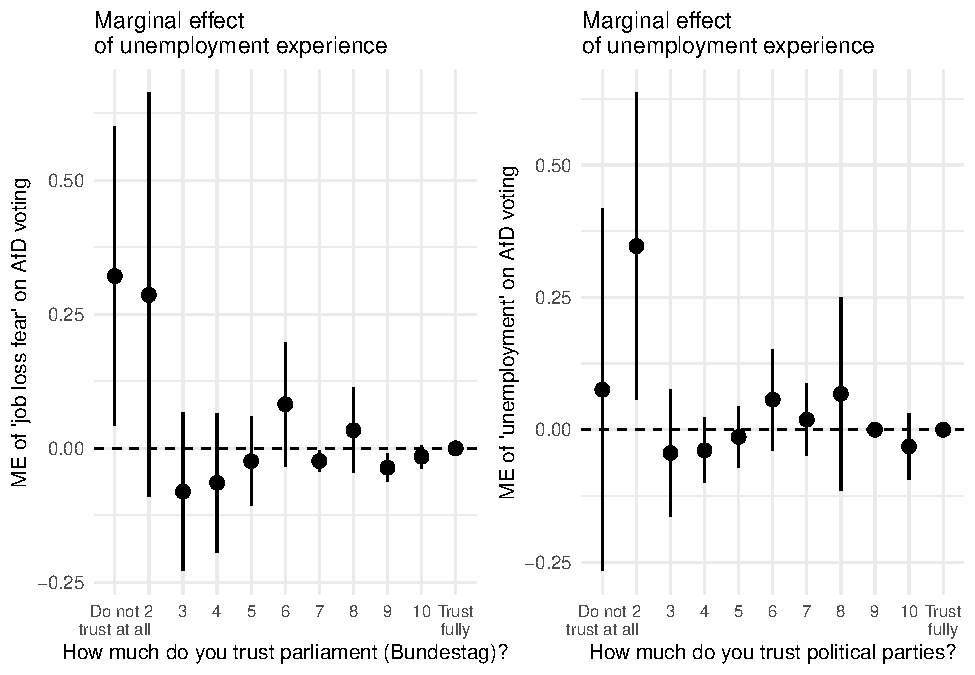
\includegraphics{AVCD_Final-Assignment-1050713_files/figure-latex/regression-results-1-plot2-1.pdf}
\caption{Marginal effects of economic insecurity by trust}
\end{figure}

\begin{table}[!h]

\caption{\label{tab:multinomial-model-table}Multinomial analysis}
\centering
\resizebox{\linewidth}{!}{
\begin{tabular}[t]{lcccccc}
\toprule
\multicolumn{1}{c}{ } & \multicolumn{6}{c}{Multinomial model with AfD as reference category} \\
\cmidrule(l{3pt}r{3pt}){2-7}
  & CDU/CSU & SPD & FDP & GRUENE/B90 & LINKE & Other party\\
\midrule
Intercept & \num{-4.157}*** & \num{-1.740}+ & \num{-0.805} & \num{-2.348}* & \num{0.976} & \num{1.210}\\
 & (\num{1.108}) & (\num{1.025}) & (\num{1.119}) & (\num{1.072}) & (\num{1.193}) & (\num{1.296})\\
Fear of job loss & \num{-0.024} & \num{-0.033} & \num{-0.076} & \num{0.019} & \num{0.034} & \num{-0.207}\\
 & (\num{0.176}) & (\num{0.166}) & (\num{0.187}) & (\num{0.172}) & (\num{0.195}) & (\num{0.244})\\
Difference which party governs & \num{0.519}*** & \num{0.289}** & \num{0.303}* & \num{0.552}*** & \num{0.156} & \num{-0.122}\\
 & (\num{0.120}) & (\num{0.111}) & (\num{0.125}) & (\num{0.122}) & (\num{0.136}) & (\num{0.142})\\
Age & \num{0.020}+ & \num{0.032}** & \num{-0.017} & \num{0.008} & \num{0.002} & \num{-0.041}**\\
 & (\num{0.012}) & (\num{0.011}) & (\num{0.012}) & (\num{0.011}) & (\num{0.013}) & (\num{0.015})\\
Female dummy & \num{0.779}** & \num{0.916}*** & \num{0.389} & \num{1.173}*** & \num{0.445} & \num{0.560}\\
 & (\num{0.280}) & (\num{0.269}) & (\num{0.297}) & (\num{0.279}) & (\num{0.326}) & (\num{0.348})\\
Household income & \num{0.210}** & \num{0.085} & \num{0.175}* & \num{0.157}* & \num{-0.017} & \num{0.141}\\
 & (\num{0.070}) & (\num{0.065}) & (\num{0.073}) & (\num{0.068}) & (\num{0.077}) & (\num{0.088})\\
Rurality of place
of residence & \num{-0.066} & \num{-0.268}* & \num{-0.206} & \num{-0.365}** & \num{-0.381}* & \num{-0.223}\\
 & (\num{0.130}) & (\num{0.124}) & (\num{0.135}) & (\num{0.128}) & (\num{0.149}) & (\num{0.160})\\
No Abitur dummy & \num{-0.585}+ & \num{-0.877}** & \num{-0.914}** & \num{-1.728}*** & \num{-1.276}*** & \num{-0.382}\\
 & (\num{0.329}) & (\num{0.317}) & (\num{0.338}) & (\num{0.324}) & (\num{0.368}) & (\num{0.398})\\
West Germany dummy & \num{1.349}*** & \num{1.556}*** & \num{1.232}*** & \num{1.967}*** & \num{0.489} & \num{0.933}**\\
 & (\num{0.281}) & (\num{0.268}) & (\num{0.296}) & (\num{0.288}) & (\num{0.320}) & (\num{0.351})\\
Num.Obs. & \num{1276} &  &  &  &  & gof\\
R2 & \num{0.589} &  &  &  &  & gof\\
R2 Adj. & \num{0.588} &  &  &  &  & gof\\
AIC & \num{4303.1} &  &  &  &  & gof\\
BIC & \num{4581.3} &  &  &  &  & gof\\
RMSE & \num{0.33} &  &  &  &  & gof\\
\bottomrule
\end{tabular}}
\end{table}

\FloatBarrier

\hypertarget{robustness-checks}{%
\subsection{Robustness checks}\label{robustness-checks}}

\begin{table}[!h]

\caption{\label{tab:regression-results1-robustness1}Robustness check I}
\centering
\begin{tabular}[t]{lcccc}
\toprule
  & (1) & (2) & (3) & (4)\\
\midrule
Fear of losing/changing profession & \num{-0.470} & \num{-1.766} &  & \\
 & (\num{0.979}) & (\num{1.661}) &  & \\
Current economic situation (subjective) &  &  & \num{0.435} & \num{0.332}\\
 &  &  & (\num{0.293}) & (\num{0.285})\\
Diff. which party one votes for &  & \num{-1.939}* &  & \num{-0.660}**\\
 &  & (\num{0.786}) &  & (\num{0.216})\\
Diff. which party governs & \num{-1.173}+ &  & \num{-0.460}* & \\
 & (\num{0.602}) &  & (\num{0.217}) & \\
Diff. which party one votes for x Fear of losing/changing profession &  & \num{0.539} &  & \\
 &  & (\num{0.411}) &  & \\
Diff. which party governs x Fear of losing/changing profession & \num{0.187} &  &  & \\
 & (\num{0.275}) &  &  & \\
Diff. which party one votes for x Current econ. situation &  &  &  & \num{0.079}\\
 &  &  &  & (\num{0.075})\\
Diff. which party governs x Current econ. situation &  &  & \num{0.052} & \\
 &  &  & (\num{0.077}) & \\
Age & \num{-0.007} & \num{-0.028} & \num{-0.005} & \num{-0.007}\\
 & (\num{0.035}) & (\num{0.037}) & (\num{0.005}) & (\num{0.006})\\
Female dummy & \num{-2.188}+ & \num{-2.521}+ & \num{-0.751}*** & \num{-0.788}***\\
 & (\num{1.286}) & (\num{1.368}) & (\num{0.181}) & (\num{0.184})\\
Household income & \num{-0.034} & \num{0.065} & \num{-0.034} & \num{-0.024}\\
 & (\num{0.172}) & (\num{0.185}) & (\num{0.040}) & (\num{0.041})\\
Rurality of place
of residence & \num{-0.118} & \num{-0.053} & \num{0.099} & \num{0.102}\\
 & (\num{0.313}) & (\num{0.315}) & (\num{0.081}) & (\num{0.082})\\
No Abitur dummy & \num{0.549} & \num{0.986} & \num{0.723}** & \num{0.698}**\\
 & (\num{0.894}) & (\num{0.930}) & (\num{0.220}) & (\num{0.222})\\
West Germany dummy & \num{-1.639}* & \num{-2.085}* & \num{-1.078}*** & \num{-1.037}***\\
 & (\num{0.825}) & (\num{0.890}) & (\num{0.175}) & (\num{0.178})\\
\midrule
Num.Obs. & \num{159} & \num{156} & \num{2417} & \num{2388}\\
AIC & \num{73.7} & \num{69.5} & \num{1032.4} & \num{1000.2}\\
BIC & \num{104.3} & \num{100.0} & \num{1090.3} & \num{1058.0}\\
Log.Lik. & \num{-26.829} & \num{-24.730} & \num{-506.198} & \num{-490.110}\\
RMSE & \num{0.21} & \num{0.21} & \num{0.24} & \num{0.23}\\
\bottomrule
\end{tabular}
\end{table}

\begin{table}[!h]

\caption{\label{tab:regression-results1-robustness2}Robustness check II}
\centering
\begin{tabular}[t]{lcccc}
\toprule
  & (1) & (2) & (3) & (4)\\
\midrule
Fear of losing/changing profession & \num{38.690} & \num{1.779} &  & \\
 & (\num{4213.436}) & (\num{1.332}) &  & \\
Current economic situation (subjective) &  &  & \num{0.603}** & \num{0.889}***\\
 &  &  & (\num{0.210}) & (\num{0.236})\\
Trust in parliament & \num{18.464} &  & \num{-0.240}* & \\
 & (\num{2106.718}) &  & (\num{0.120}) & \\
Trust in parties &  & \num{0.346} &  & \num{-0.178}\\
 &  & (\num{0.609}) &  & (\num{0.156})\\
Trust in parliament x Fear of losing/changing profession & \num{-18.899} &  &  & \\
 & (\num{2106.718}) &  &  & \\
Trust in parties x Fear of losing/changing profession &  & \num{-0.612} &  & \\
 &  & (\num{0.500}) &  & \\
Trust in parliament x Current econ. situation &  &  & \num{-0.102}* & \\
 &  &  & (\num{0.047}) & \\
Trust in parties x Current econ. situation &  &  &  & \num{-0.146}*\\
 &  &  &  & (\num{0.060})\\
Age & \num{-0.023} & \num{-0.020} & \num{0.003} & \num{-0.002}\\
 & (\num{0.047}) & (\num{0.039}) & (\num{0.006}) & (\num{0.006})\\
Female dummy & \num{-20.322} & \num{-17.727} & \num{-0.898}*** & \num{-0.947}***\\
 & (\num{8816.272}) & (\num{2112.882}) & (\num{0.201}) & (\num{0.202})\\
Household income & \num{0.436} & \num{0.027} & \num{-0.028} & \num{-0.027}\\
 & (\num{0.339}) & (\num{0.191}) & (\num{0.046}) & (\num{0.044})\\
Rurality of place
of residence & \num{0.205} & \num{0.086} & \num{0.135} & \num{0.097}\\
 & (\num{0.367}) & (\num{0.314}) & (\num{0.088}) & (\num{0.086})\\
No Abitur dummy & \num{1.168} & \num{0.632} & \num{0.674}** & \num{0.787}***\\
 & (\num{1.082}) & (\num{0.985}) & (\num{0.233}) & (\num{0.230})\\
West Germany dummy & \num{-1.391} & \num{-1.445} & \num{-1.050}*** & \num{-1.116}***\\
 & (\num{0.997}) & (\num{0.886}) & (\num{0.188}) & (\num{0.188})\\
\midrule
Num.Obs. & \num{155} & \num{156} & \num{2351} & \num{2341}\\
AIC & \num{56.5} & \num{64.8} & \num{865.1} & \num{885.4}\\
BIC & \num{86.9} & \num{95.3} & \num{922.8} & \num{943.0}\\
Log.Lik. & \num{-18.228} & \num{-22.388} & \num{-422.563} & \num{-432.693}\\
RMSE & \num{0.19} & \num{0.20} & \num{0.22} & \num{0.22}\\
\bottomrule
\end{tabular}
\end{table}

\FloatBarrier

\hypertarget{references}{%
\section*{References}\label{references}}
\addcontentsline{toc}{section}{References}

\hypertarget{refs}{}
\begin{CSLReferences}{1}{0}
\leavevmode\vadjust pre{\hypertarget{ref-art_myth_2022}{}}%
Art, David. 2022. {``The {Myth} of {Global} {Populism}.''}
\emph{Perspectives on Politics} 20 (3): 999--1011.

\leavevmode\vadjust pre{\hypertarget{ref-arzheimer_how_2019}{}}%
Arzheimer, Kai, and Carl C. Berning. 2019. {``How the {Alternative} for
{Germany} ({AfD}) and Their Voters Veered to the Radical Right,
2013--2017.''} \emph{Electoral Studies} 60 (August): 102040.

\leavevmode\vadjust pre{\hypertarget{ref-autor_china_2013}{}}%
Autor, David H, David Dorn, and Gordon H. Hanson. 2013. {``The {China}
{Syndrome}: {Local} {Labor} {Market} {Effects} of {Import} {Competition}
in the {United} {States}.''} \emph{American Economic Review} 103 (6):
2121--68.

\leavevmode\vadjust pre{\hypertarget{ref-autor_unexpected_2023}{}}%
Autor, David H, Arindrajit Dube, and Annie McGrew. 2023. {``The
{Unexpected} {Compression}: {Competition} at {Work} in the {Low} {Wage}
{Labor} {Market}.''} Working \{Paper\}. Working {Paper} {Series}.
National Bureau of Economic Research.
\url{https://doi.org/10.3386/w31010}.

\leavevmode\vadjust pre{\hypertarget{ref-becker_2020_separation}{}}%
Becker, Sascha O, Lukas Mergele, and Ludger Wößmann. 2020. {``The
Separation and Reunification of Germany: Rethinking a Natural Experiment
Interpretation of the Enduring Effects of Communism.''} \emph{Journal of
Economic Perspectives} 34 (2): 143--71.

\leavevmode\vadjust pre{\hypertarget{ref-boix_democratic_2019}{}}%
Boix, Carles. 2019. \emph{Democratic {Capitalism} at the {Crossroads}:
{Technological} {Change} and the {Future} of {Politics}}. Illustrated
Edition. Princeton: Princeton Univers. Press.

\leavevmode\vadjust pre{\hypertarget{ref-cantoni_persistence_2020}{}}%
Cantoni, Davide, Felix Hagemeister, and Mark Westcott. 2020.
{``Persistence and {Activation} of {Right}-{Wing} {Political}
{Ideology}.''}
\url{http://www.davidecantoni.net/pdfs/afd_draft_20200512.pdf}.

\leavevmode\vadjust pre{\hypertarget{ref-colantone_trade_2018}{}}%
Colantone, Italo, and Piero Stanig. 2018a. {``The {Trade} {Origins} of
{Economic} {Nationalism}: {Import} {Competition} and {Voting} {Behavior}
in {Western} {Europe}.''} \emph{American Journal of Political Science}
62 (4): 936--53.

\leavevmode\vadjust pre{\hypertarget{ref-colantone_global_2018}{}}%
---------. 2018b. {``Global {Competition} and {Brexit}.''}
\emph{American Political Science Review} 112 (2): 201--18.

\leavevmode\vadjust pre{\hypertarget{ref-colantone_surge_2019}{}}%
---------. 2019. {``The {Surge} of {Economic} {Nationalism} in {Western}
{Europe}.''} \emph{Journal of Economic Perspectives} 33 (4): 128--51.

\leavevmode\vadjust pre{\hypertarget{ref-cziriak_publication_nodate}{}}%
Cziriak, Marius. 2022. {``{Households}' {Financial} {Fragility} {During}
the {COVID}-19 {Pandemic} in {Germany}.''} {ZEW} {Discussion} {Paper}.
\url{https://www.zew.de/en/publications/households-financial-fragility-during-the-covid-19-pandemic-in-germany-1}.

\leavevmode\vadjust pre{\hypertarget{ref-dauth_rise_2014}{}}%
Dauth, Wolfgang, Sebastian Findeisen, and Jens Südekum. 2014. {``The
{Rise} of the {East} and the {Far} {East}: {German} {Labor} {Markets}
and {Trade} {Integration}.''} \emph{Journal of the European Economic
Association} 12 (6): 1643--75.

\leavevmode\vadjust pre{\hypertarget{ref-dauth_adjustment_2021}{}}%
Dauth, Wolfgang, Sebastian Findeisen, Jens Südekum, and Nicole Wößner.
2021. {``The {Adjustment} of {Labor} {Markets} to {Robots}.''}
\emph{Journal of the European Economic Association} 19 (6): 3104--53.

\leavevmode\vadjust pre{\hypertarget{ref-dustmann_europes_2017}{}}%
Dustmann, Christian, Barry Eichengreen, Sebastian Otten, André Sapir,
Guido Tabellini, and Gylfi Zoega. 2017. {``Europe's {Trust} {Deficit}:
{Causes} and {Remedies}.''} London: Centre for Economic Policy Research.
\url{http://www.christiandustmann.com/content/4-research/14-europe-s-trust-deficit-causes-and-remedies/europe-s-trust-deficit-causes-and-remedies.pdf}.

\leavevmode\vadjust pre{\hypertarget{ref-eichengreen_populist_2018}{}}%
Eichengreen, Barry. 2018. \emph{The {Populist} {Temptation}: {Economic}
{Grievance} and {Political} {Reaction} in the {Modern} {Era}}. New York,
NY: Oxford University Press.

\leavevmode\vadjust pre{\hypertarget{ref-green_politics_2017}{}}%
Green, Jane, and Will Jennings. 2017. \emph{The {Politics} of
{Competence}: {Parties}, {Public} {Opinion} and {Voters}}. Cambridge,
UK: Cambridge University Press.

\leavevmode\vadjust pre{\hypertarget{ref-guriev_political_2022}{}}%
Guriev, Sergei, and Elias Papaioannou. 2022. {``The {Political}
{Economy} of {Populism}.''} \emph{Journal of Economic Literature} 60
(3): 753--832.

\leavevmode\vadjust pre{\hypertarget{ref-haffert_stadt_2022}{}}%
Haffert, Lukas. 2022. \emph{Stadt, {Land}, {Frust}: {Eine} Politische
{Vermessung}}. München: C.H.Beck.

\leavevmode\vadjust pre{\hypertarget{ref-ivanov_economic_2023}{}}%
Ivanov, Denis. 2023. {``Economic {Insecurity}, {Institutional} {Trust}
and {Populist} {Voting} {Across} {Europe}.''} \emph{Comparative Economic
Studies}, February.

\leavevmode\vadjust pre{\hypertarget{ref-katz_cartel_2009}{}}%
Katz, Richard S., and Peter Mair. 2009. {``The {Cartel} {Party}
{Thesis}: {A} {Restatement}.''} \emph{Perspectives on Politics} 7 (4):
753--66.

\leavevmode\vadjust pre{\hypertarget{ref-kitschelt_radical_1995}{}}%
Kitschelt, Herbert, and Anthony J. McGann. 1995. \emph{The {Radical}
{Right} in {Western} {Europe}: {A} {Comparative} {Analysis}}. Michigan:
University of Michigan Press.

\leavevmode\vadjust pre{\hypertarget{ref-linz_breakdown_1978}{}}%
Linz, Juan J. 1978. \emph{The {Breakdown} of {Democratic} {Regimes}:
{Crisis}, {Breakdown} and {Reequilibration}. {An} {Introduction}}.
Baltimore: Johns Hopkins University Press.

\leavevmode\vadjust pre{\hypertarget{ref-manow_ent-demokratisierung_2020}{}}%
Manow, Philip. 2020. \emph{({Ent}-){Demokratisierung} Der {Demokratie}}.
Berlin: Suhrkamp Verlag.

\leavevmode\vadjust pre{\hypertarget{ref-margalit_economic_2019}{}}%
Margalit, Yotam. 2019. {``Economic {Insecurity} and the {Causes} of
{Populism}, {Reconsidered}.''} \emph{The Journal of Economic
Perspectives} 33 (4): 152--70.

\leavevmode\vadjust pre{\hypertarget{ref-margalit_cultural_2022}{}}%
Margalit, Yotam, Shir Raviv, and Omer Solodoch. 2022. {``The {Cultural}
{Origins} of {Populism}.''} Rochester, NY.
\url{https://doi.org/10.2139/ssrn.4001543}.

\leavevmode\vadjust pre{\hypertarget{ref-milner_voting_2021}{}}%
Milner, Helen V. 2021. {``Voting for {Populism} in {Europe}:
{Globalization}, {Technological} {Change}, and the {Extreme} {Right}.''}
\emph{Comparative Political Studies} 54 (13): 2286--2320.

\leavevmode\vadjust pre{\hypertarget{ref-plumper_strategy_2021}{}}%
Plümper, Thomas, Eric Neumayer, and Katharina Gabriela Pfaff. 2021.
{``The Strategy of Protest Against {Covid}-19 Containment Policies in
{Germany}.''} \emph{Social Science Quarterly} 102 (5): 2236--50.

\leavevmode\vadjust pre{\hypertarget{ref-schafer_demokratische_2021}{}}%
Schäfer, Armin, and Michael Zürn. 2021. \emph{Die Demokratische
{Regression}}. Berlin: Suhrkamp Verlag.

\leavevmode\vadjust pre{\hypertarget{ref-silva_parties_2023}{}}%
Silva, Bruno Castanho, and Christopher Wratil. 2023. {``Do Parties'
Representation Failures Affect Populist Attitudes? {Evidence} from a
Multinational Survey Experiment.''} \emph{Political Science Research and
Methods} 11 (2): 347--62.

\leavevmode\vadjust pre{\hypertarget{ref-sonin_historical_2022}{}}%
Sonin, Konstantin. 2022. {``The {Historical} {Perspective} on the
{Donald} {Trump} {Puzzle}: {A} {Review} of {Barry} {Eichengreen}'s
"{The} {Populist} {Temptation}: {Economic} {Grievance} and {Political}
{Reaction} in the {Modern} {Era}".''} \emph{Journal of Economic
Literature} 60 (3): 1029--38.

\end{CSLReferences}

\end{document}
